% NeuroCam manual - GPIO/Synch Boxes
% Written by Christopher Thomas.
% Copyright (c) 2021 by Vanderbilt University. This work is released under
% the Creative Commons Attribution-ShareAlike 4.0 International License.

\chapter{GPIO and Synch Box}
\label{gpio}

The GPIO-and-synch box provides TTL-level inputs via a rectangular connector
and TTL-level synchronization outputs via BNC connectors. Changes to inputs
are reported to the NeuroCam computer via USB cable.

During normal operation of the NeuroCam system, the following functions are
performed:
\begin{itemize}
\item The synchronization lines are strobed high for 20~ms every 10 seconds,
with changes in the outputs recorded in session log files.
\item Changes to TTL inputs are recorded in session log files.
\item Low-to-high transitions on input bits 7 and 6 cause the NeuroCam to
start and stop recording a session, respectively. There is a ``dead time''
of 10 seconds between successive commands being recognized.
\end{itemize}

The front panel and interior of a GPIO-and-synch box are shown below:

\begin{center}
% The exterior image is 800x600, the interior is 600x600.
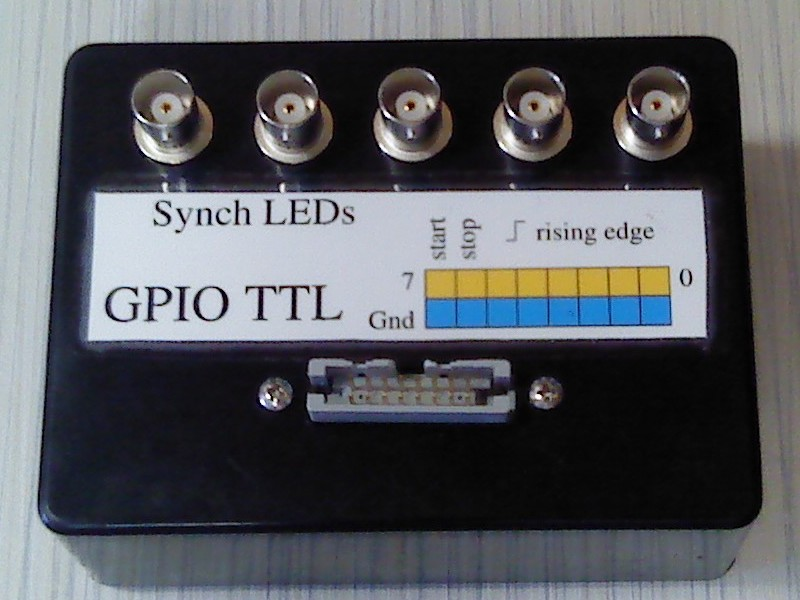
\includegraphics[height=2in]{pics-gpio/gpio-closed.jpg}
\hspace{1in}
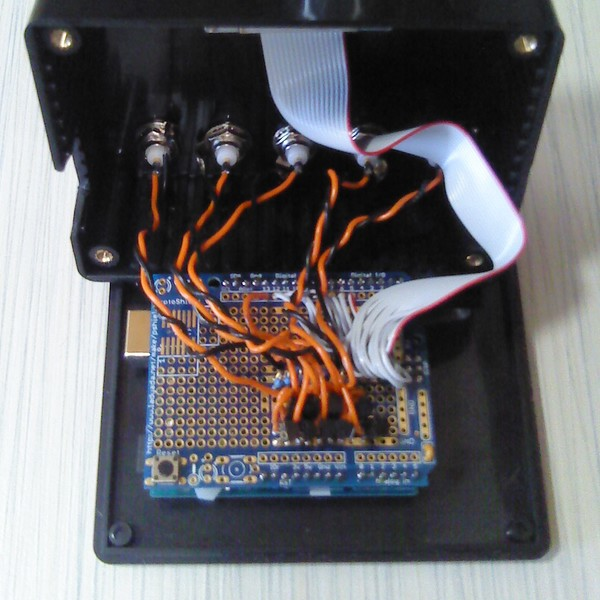
\includegraphics[height=2in]{pics-gpio/gpio-open.jpg}
\end{center}

\clearpage
The parts needed for a GPIO-and-synch box are as follows:

\begin{tabular}{llll}\hline
Qty & Description & Manuf. p/n & Digikey p/n \\
\hline
%
1 & Arduino Uno rev3 & A000066 & 1050-1024-ND \\
1 & Arduino prototyping shield kit & 2077 & 1528-1207-ND \\
9 & NFET TO-92 & BS170 & BS170-ND \\
3 & resistor 4.75 kohm 0.25w & MFR-25FBF52-4K75 & 4.75KXBK-ND \\
7 & resistor 475 ohm 0.25w & MFR-25FBF52-475R & 475XBK-ND \\
5 & BNC jack panel mount & 31-221-RFX & ARFX1064-ND \\
1 & box abs 4.3x3.2x1.7 & 1591SBK & HM121-ND \\
1 & conn 16 pin female to ribbon & M1YXK-1636J & M1YXK-1636J-ND \\
2 & machine screw 4-40 0.5in ss & 9902 & 36-9902-ND \\
2 & hex nut 4-40 ss & 7248-3 & 36-7248-3-ND \\
4 & machine screw 4-40 0.375in nylon & 9528 & 36-9528-ND \\
4 & hex nut 4-40 nylon & 9605 & 36-9605-ND \\
1 & USB cable male A to male B & 102-1030-BE-00200 & 1175-1089-ND \\
%
\hline
\end{tabular}

\textbf{NOTE:} The prototyping shield kit includes male pin headers,
one female ISP header, two decoupling capacitors, one pushbutton switch,
one red LED, and one green LED, which are required for the GPIO-and-synch
box.

The prototyping shield kit should be assembled per its directions. There are
several important things to keep in mind:
\begin{itemize}
%
\item The pin headers (including ISP header) should be plugged into an
Arduino Uno, with the prototyping shield board friction-seated on the header
pins, prior to soldering. This guarantees proper mechanical alignment of the
headers.
%
Do not use the long-tail female ``stacking'' headers for I/O pins. These
do not mate properly with the Arduino Uno. The only female header used is
for the ISP header connection.
%
\item The two decoupling capacitors should be soldered in their marked
positions on the board.
%
\item Only one of the two provided switches is used. This is soldered to
the ``reset switch'' location indicated on the board.
%
\item The red and green 3mm LEDs are not soldered to the prototyping board.
They are used for strobe and power lights on the front panel of the
GPIO-and-synch box if such lights are desired. They mount in 1/8" holes,
and should be secured in place using epoxy on their rear sides.
%
\end{itemize}

\clearpage
The following circuit should be built on the prototyping shield:

\begin{center}
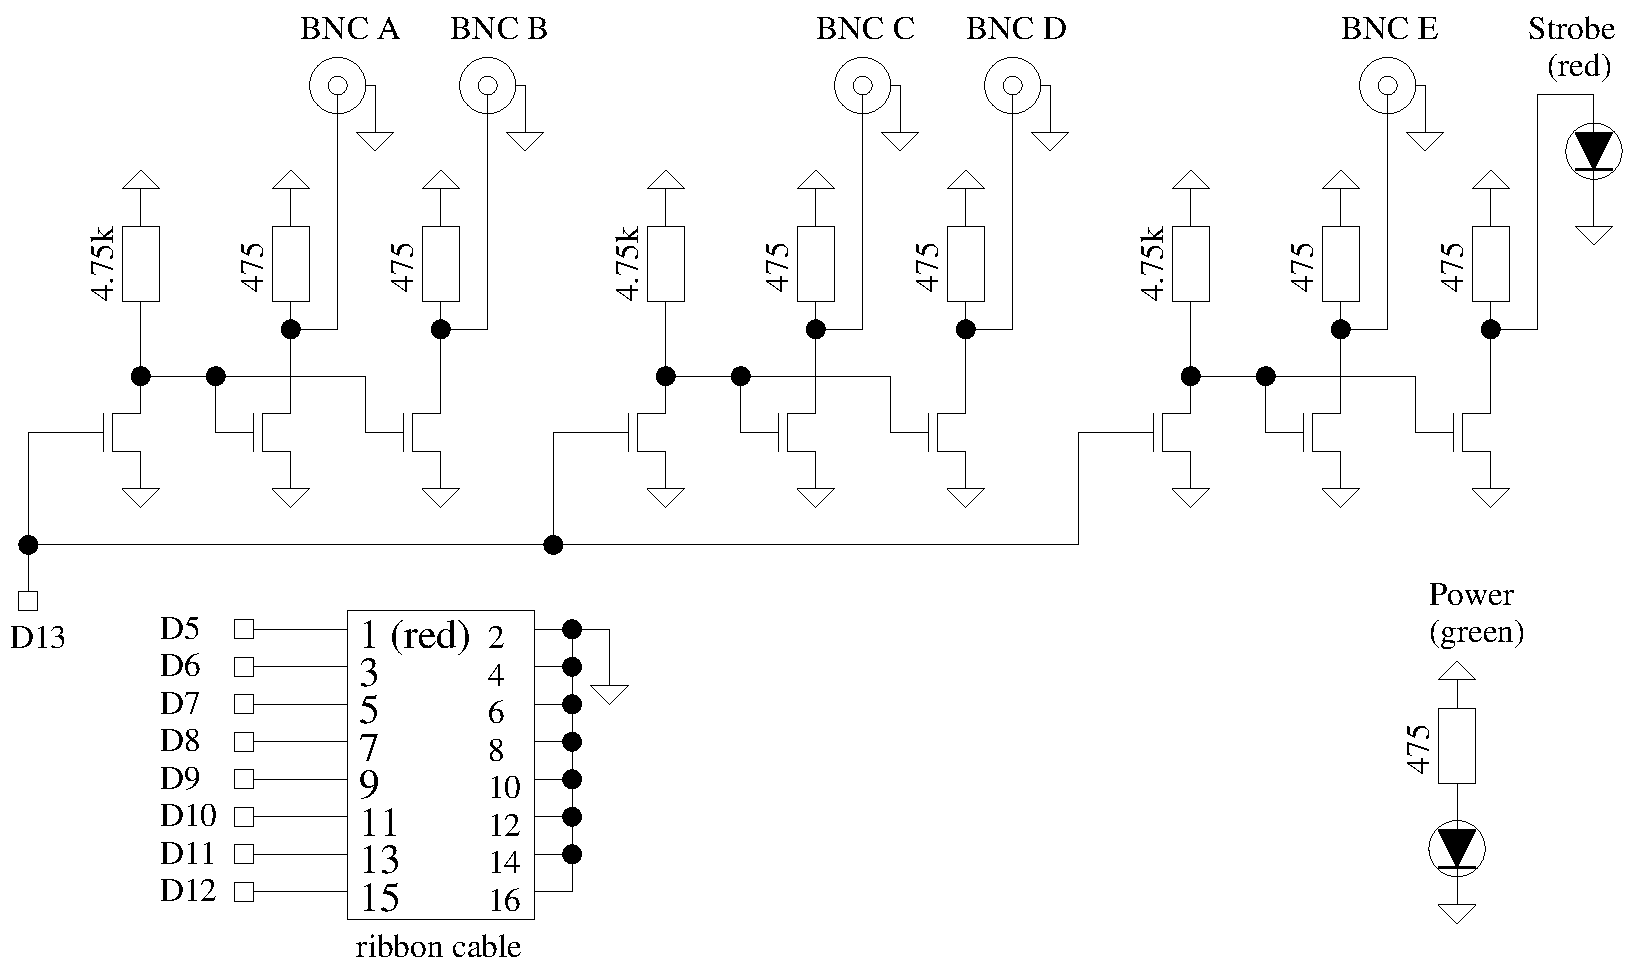
\includegraphics[width=0.9\textwidth]{drawings/gpio-dev-schem.pdf}
\end{center}

A mechanical drawing of the front panel is as follows:

\begin{center}
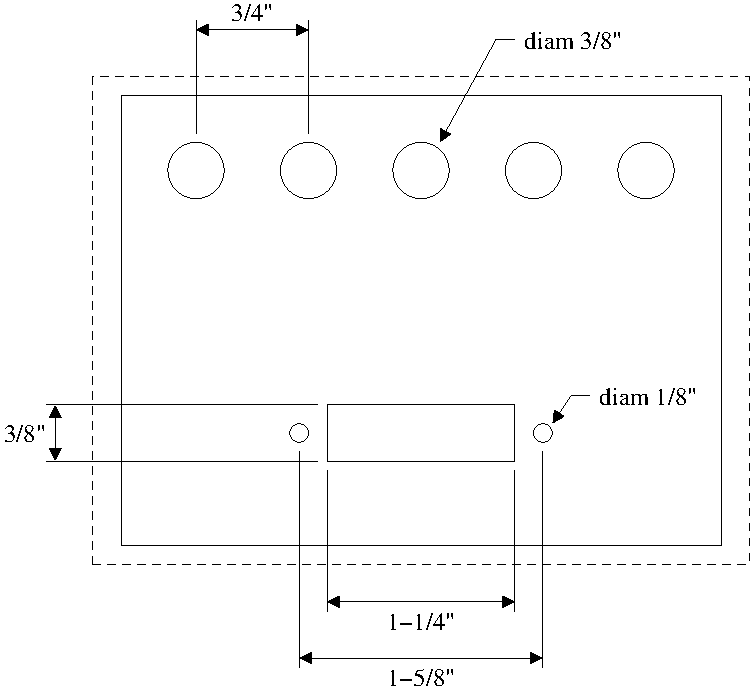
\includegraphics[height=3in]{drawings/gpio-dev-front-mech.pdf}
\end{center}

The rear panel should have mounting holes compatible with the Arduino Uno
(1/8", countersunk).

%
% This is the end of the file.
